\documentclass{article}
\usepackage[hidelinks]{hyperref}
\usepackage{apacite}
\usepackage{graphicx}
\usepackage{a4wide}
\usepackage{booktabs}
\usepackage{rotating}
\usepackage[nonumberlist]{glossaries}

\bibliographystyle{apacite}
\makeglossaries
\newacronym{MSP}{MSP}{Metagenomic Species Pan-genomes}
\newacronym{CAG}{CAG}{Co-Abundance gene Groups}
\newacronym{CPU}{CPU}{Central Processing Unit}
\newacronym{MAG}{MAG}{Metagenome-Assembled Genome}
\newacronym{VAMB}{VAMB}{Variational Autoencoders for Metagenomic Binning}

% For drafts
\usepackage{setspace}
\doublespacing
\usepackage{lineno}
\linenumbers

\title{Metagenomic Binning Pipelines - the State of the Art}
\date{}
\begin{document}
\maketitle

\tableofcontents

\section{Abstract}
New generations of sequencing platforms coupled with numerous bioinformatics tools have led to rapid technological progress in metagenomics to investigate complex microorganism communities.
Nevertheless, a combination of different bioinformatic tools remains necessary to draw conclusions out of microbiota studies.
As sequencing costs have dropped at a rate above 'Moore's law', a greater number of large data sets are being produced than ever before.
Newer algorithms that take advantage of the size of these datasets are continually being developed.
Binning algorithms are defined as the grouping of assembled metagenomic contigs by their genome of origin (\autoref{Fsummary}).
Selecting the most appropriate binning algorithm can be a daunting task and is influenced by many factors.
This review serves as a guide to direct the researcher to the binning algorithm that best suits their needs.

\begin{figure}
\centering
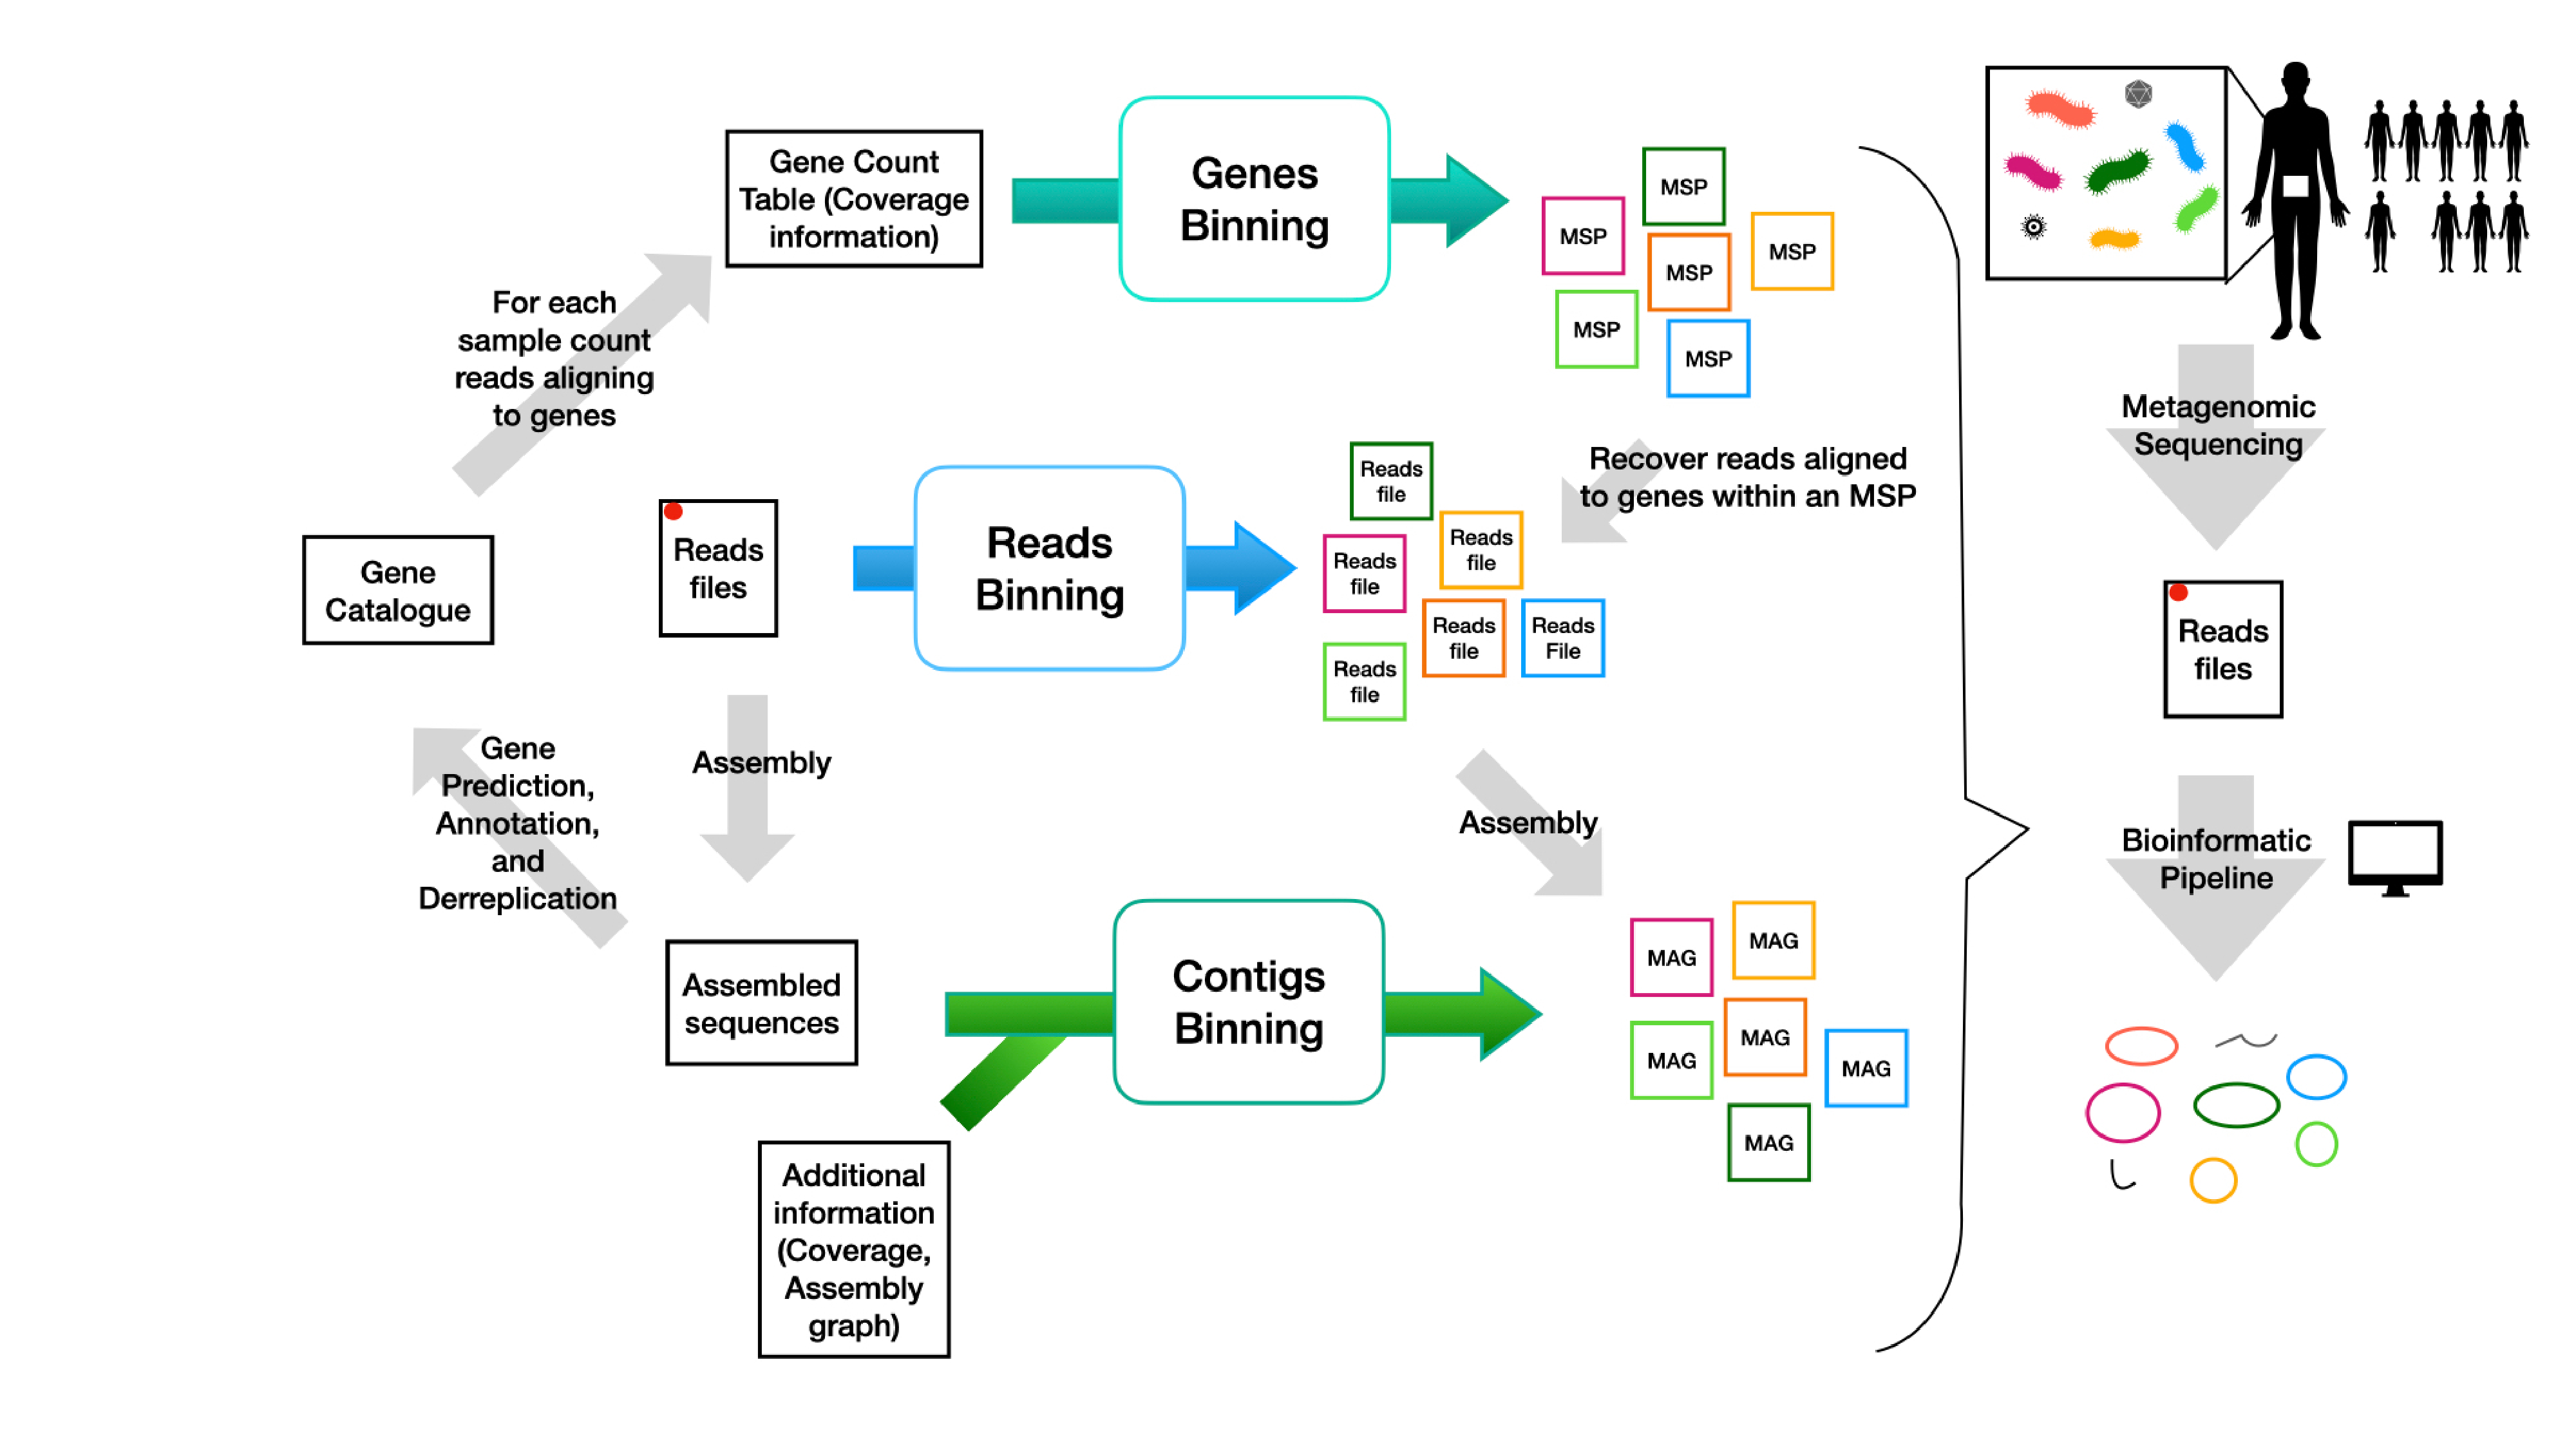
\includegraphics[scale=0.2]{figures/figure_binning_software.001.pdf}
\caption["Summary of binning principles and techniques"]{
	Summary of binning principles and techniques.}
\label{Fsummary}
\end{figure}

\section{Background}
%Binning problem definition (recover biological entities from metagenomic sequencing)
%problem relevance (Explosion in metagenomics, reduction in sequencing cost, increased computer capacity)
%Review objectives (Brief summary on popular tools, innovations overview of recent tools)
The explosion in popularity and success in the field of metagenomics over the last 25 years can be largely attributed to the advances in computing technologies.
An example of the outcomes of this can be found in the Human Microbiome Project; a project that has been greatly improved the understanding of the microbila flora involved in human health and disease.
These advances have brought with them greater demands for storage, CPU time, and consequently more efficient algorithms.
The main function of binning tools is to reconstruct species/biological entities from metagenomic samples.  
Compared to amplicon, shotgun metagenome can provide functional gene profiles directly and reach a much higher resolution of taxonomic annotation.
However, due to the high demands on computational resources, cost, and expertise necessary to perform this analysis, researchers have historically been limited in their capacity to collect and analyse sequencing data.
As the cost of sequencing is rapidly falling, this burden has been significantly lessened.
Whole Genome Shotgun sequences does not require cultivation.
At the time of writing, shotgun metagenomic sequencing costs on average three times as much as 16S sequencing in comparison.
%The objectives of this review is for the reader to be better informed about the latest algorithms (since 2017) for binning metagenomic samples.
%The second part of this review is for the reader to be informed about distinguishing factors between the methods.
%The last part is for the reader to make an informed decision based on those factors for their needs.
%This review will be broken down into the following sections:
Here we will briefly recapitulate recent binning algorithms and highlight some of the developments in the field, among them, the use of new algorithms and strategies employed to achieve the goal of identifying the organisms composing microbiome communities.
We hope this overview could aid the reader to choose a binning algorithm or a combination of them based on their specific needs.

\section{Overview of recent methods for metagenomic binning}
\subsection{Progress in recent binning strategies}
%Proposed solutions (bin contings into bins(MAG if good quality) based on their kmer composition and abundance/coabundance)
%Tools available (Cite recent benchmark)} 
%Read binning 
%gene-abundance binning (CAG, MGS, MSPi)
%Integrate new experimental data 
%Figure. Binning software historical citations barplot 

A metagenomic sample is comprised of many organisms and the goal of binning is to reconstruct the sequences from each organism present in the original sample.
The majority of binning tools we can find are oriented toward clustering contigs (contig-binning) into bins, which may represent the genome from a single biological entity/organism. A \gls{MAG} is a single-taxon assembly based on one or more binned metagenomes that has been asserted to be a close representation to an actual individual genome (that could match an already existing isolate or represent a novel isolate).

Current contig-binning tools normally are reference free (i.e do not depend on reference sequences to perform clustering) and rely on coverage information and sequence composition.
Progress in contig-binning algorithms can be seen in the proposals to integrate new sources of information (for example, from scaffold-graphs(Binnacle), paired-end reads(COCACOLA), or 3D contact information(MetaTOR)) and state of the art algorithms in machine learning (CoCoNet, \gls{VAMB}).

We also notice the development of Bin refinement tools (DAS-tool, Binning Refiner), this tools rely on the outputs from multiple contig-binning algorithms and attempt to combine them to produce better results.

Binning of contigs have played a central role in software development in the field, a review on the benchmarking binning algorithms was done by \citeNP{yue2020evaluating}. 
%Currently we can distinguish from 3 different stategies in binning algorithms, read binning, contig binning, and gene binning.

Beside contig-binning tools we can also distinguish read-binning tools and co-abundant-gene-binning tools.

The main purpose of read-binning tools is to pre-process reads into clusters for a posterior targeted assembly, here we find reference-free and non-reference-free tools, and tools designed for short-read or long-read sequencing technologies. Among the binning tools developed in recent years a subset of them are dedicated to cluster reads (read-binning) (MetaBBC-LR, BioBloom Tools, CLAME, LVQ-KKN, Meta VW, HirBin, MEGAN-LR).

%\subsubsection{Metagenome Assembled Genomes}
\subsubsection{ binning co-abundant genes}
Binning of co-abundant genes represents an alternative proposal to reconstruct species/biological entities from a set of metagenomic samples.
Co-abundant gene binning methods assume each gene coming from a shared chromosome will display proportional abundances across samples, if you have enough samples from a similar environment you can identify the sets of genes from a common organism of origin (MLGs Chameleon-clust 2012, CAGs and MGSs Canopy 2014, Markovclust-MGCs Karlsson 2013, MSPs MSPminner 2018).
In the past few years the MSPminer software was developed exploiting this approach. MSPminer introduced a robust proportionality measure detecting co-abundant but no necessarily co-occurring.
This tools groups co-abundant genes into Metagenomic Species Pan-genomes or \glspl{MSP} and classify genes within an MSP as core, accessory and shared. Core genes are present in all strains, accessory are present only in some(Medini et al., 2005), the shared category applies for those genes which may be present in more than one MSP due to horizontal transfer.
%Microbial pan-genomes are gene repertoires composed of core genes present in all strains and accessory genes present in only some of them (Medini et al., 2005).
The factors that impact directly on \gls{MSP} quality include the sample composition, the sequencing depth, the previous bioinforamtic steps to build the reference gene dataset and to map the reads.
%A high number of samples with varying phenotypes improve the quality of \glspl{MSP}.
MSPs can be employed for taxonomic profiles of new samples from similar ecosystems at the species level, and also to compare strains between samples building a presence/absence table of accessory genes and for biomarker discovery.
By binning contigs carrying genes from the same MSP it is also possible to build a \gls{MAG}.

%\subsubsection{Metagenomic Species Pan-genomes}
%In a shotgun metagenomic sequencing context, we define as shared the genes detected in some samples where the species is not present.
%A strain found in a sample is an instance of the species pan-genome: it is made of all the species (shared) core genes and of a subset of (shared) accessory genes. Core genes are suitable for taxonomic profiling at species-level while accessory genes can be used to compare strains across samples. Genes tagged as shared should be used carefully as they contain false positives counts or are subject to horizontal transfer.
%Core genes are suitable for taxonomic profiling at species-level while accessory genes can be used to compare strains across samples.
%Genes tagged as shared should be used carefully as they contain false positives counts or are subject to horizontal transfer.

\subsubsection{Binning microbial genomes with deep learning}
The integration of deep learning techniques into the field of metagenomics has revolutionised the field of metagenomics. The Software VAMB and CoCoNet constitute two such examples in the binning area.
%The \gls{VAMB} pipeline was developed to take advantage of variational autoencoders; a generative machine learning model that uses a deep variational autoencoders \cite{nissenimproved}...
%COCONET \cite{arisdakessian2021coconet}...

The main feature VAMB is the application of the Deep Learning technique knwon as Variational Auto Encoders (VAE). The variational autoencoders in VAMB learn how to integrate two data types, coabundance and kmer composition. The reulting latent representation clusters better than either of the inputs, but in principe is not limited by only two data types, and it would be possible to incorpoate more data as input to the VAE.
VAMB also applies a "mulitsplit" approach where each cluster should correpond to an organism representation across samples and each bin in a cluster to a per-sample representation of the genome of that orgamisn.
Deep learning approaces also benefit from the fact GPU technology has advanced rapidly over the past few years.

The CoCoNet software uses deep learning and clustering to bin contigs into clusters representing species present in the samples. The algorithm consists in two phases, the first phase train a neural network to estimate the probability that two contigs come from the same genome, given their composition and coverage information. The second use a heuristic to bin the contigs using the probabilities inferred in the first stage
An interesting feature in CoCoNet is it was trained on viral genomes. In the following section we discuss more about binning on viral genomes. 

\subsection{Binning of viral genomes}
%Endosymbionts 
%2021 viral catalog \cite{nayfach2021metagenomic}...
%New insights from uncultivated genomes of the global human gut microbiome \cite{nayfach2019new}...
%Also mention coconet suitability for viral genomes...

Most binning algorithms are designed for prokariotic organisms leaving viruses out of the software scope. Viruses important for many reasons, thus it was not unexpected binning algorithms focusing on sequences of viral origin also have shown some progress. 

CoCoNet uses deep leaning to model co-ocurrence of contigs from the same viral genome. The network was optimized for diverse viral metagenomes, the network learns to model coverage variability within samples, a critical feature in viral metagenomes where DNA amplification methods are needed to increase input genetic material.

VirBin clusters contigs for genome reconstruction of viral strains, different strains within viral species may show different biological properties such as transmissibility or virulence. Composition based features are usually are not enough to separate haplotypes, VirBin receives contigs as inputs and outputs the estimated number of haplotypes via contig aligment and returns the contigs for each haplotype based on relative abundance distribution, when the contigs are long enough VirBin produce better results.

Newer strategies has been proposed and employed to reconstruct viral genomes from metagenomic samples, in a recent work (Natfach 2021) a new compendium of 189680 DNA viruses from the human gut microbiome was produced. In this work they use viral informative features, among them are presence of viral protein families (Paez-Espino 2016), and absence of non-viral families (El Gebali 2019), gene strand switch rate (Roux 2015) and the score produced from the VirFinder(Ren et al 2017) software  

\subsection{ Binning Pipelines}
%An analysis pipeline is defined as a program that combines several programs in a defined order to complete a complex analysis.
Other advances in binning consist in the integration of existing tools and software into bioinformatic pipelines, which  allow the automatic processing from beginning to end of read samples into bins or the addition of extra processing steps to address specific biological questions or problems related to the sample of origin.

%nf-core MAG,
%MetaWRAP
%MAGO
%Autometa

MetaWRAP is a modular pipeline ready to perform common tasks in metagenomic analysis, starting from read quality checks up to bin creation, refinement, reassembly quantification, taxonomic annotation and functional annotation.
MAGO pipeline integrates metagenome assembly, binning, bin improvement, bin quality check, bin functional annotation, and bin taxonomic annotation. 
SqueezeMeta also integrates external software to perform the complete analysis of metagenomic samples from sequences reading to MAG construction and annotation.%Binning refiner
nf-coreMAG supports both short and long reads, performs quality and adapter trimming, quality check,  performs assembly, binning, checks bin quality and assigns taxonomy.

Autometa was developed to deal with non-model Eukariotic host contamination and complex single metagenomes, the application integrate sequence homology, nucleotide composition, coverage and single-copy marker genes to separate microbial genomes from non model host genomes. 
Seqdex is a tool written in R which tries to separate endosymbionts from their host sequences, they propose the use specific features in endosymbiotic systems to better solve this problem. This tool combines partial taxonomic annotations obtained trough homology searches and sequence composition to predict the contig's organism of origin from host and its endosymbionts and helps the user to understand how effective is the classification.

Among pipelines benefits we can mention they ease the reproducibility and scalability of metagenomic analysis, and they allow people with little computational experience to perform complete analysis in less time.

\section{Some suggestions on choosing a binning algorithm}
%Figure. Decision tree, overview of metagenomic binning 
\begin{sidewaystable}
\begin{tiny}
\centering
\caption[Comparison of binning algorithms]{Comparison of binning algorithms}
	\begin{tabular}{lrlllr}
\toprule
        Software/Algorithm &  Year &                                Description/purpose &                                  Comment/Highlight &                            Doi &  PubmedID \\
\midrule
                   CoCoNet &  2021 &    Deep learning tool for Viral Metagenome Binning &                          Reconstucts viral genomes & 10.1093/bioinformatics/btab213 &  33822891 \\
                  Binnacle &  2021 & Using scaffolds to improve Metagenomic bin quality &                  Incorporates scaffold information &      10.3389/fmicb.2021.638561 &  33717033 \\
                      VAMB &  2021 & Metagenome binning using deep variational autoe... &            Autoencoder algorithm, fast processing  &     10.1038/s41587-020-00777-4 &  33398153 \\
                phyloFlash &  2020 &                  ssrRNA profiling and MAG assembly & incorporates ssrRNA profiling info into MAG ass... &      10.1128/mSystems.00920-20 &  33109753 \\
                MetaBCC-LR &  2020 &                 Metagenomic binning for Long-Reads &      Suitable for Long Reads sequencing technology & 10.1093/bioinformatics/btaa441 &  32657364 \\
            BioBloom Tools &  2020 & Reads binning for targeted assembly, alignment ... & Data preparation for targeted assembly, using s... &        10.1073/pnas.1903436117 &  32641514 \\
                  GraphBin &  2020 & Refined binning of metagenomic contigs using as... &           Incorporates assembly graphs information & 10.1093/bioinformatics/btaa180 &  32167528 \\
                MetaSIPSim &  2020 & Simulating metagenomic stable isotope probing d... & Augment binning resolution with extra experimen... &      10.1186/s12859-020-3372-6 &  32000676 \\
                   MetaCon &  2019 & Unsupervised binning k-mers and coverage, focus... &                    Focus different lengths contigs &      10.1186/s12859-019-2904-4 &  31757198 \\
                    VirBin &  2019 &    Binning viral haplotypes from assembled contigs &                              Viral haplotypes MAGs &      10.1186/s12859-019-3138-1 &  31684876 \\
MAGO (*only tool pipeline) &  2019 &      Framework for Production and analysis of MAGs &                                           pipeline &          10.1093/molbev/msz237 &  31633780 \\
                    SeqDex &  2019 & Genome separation of Endosymbionts from mixed s... &                     Identification of endosymbiont &       10.3389/fgene.2019.00853 &  31608107 \\
                   MetaTOR &  2019 & High quality MAGs from mammalian guts using met... &                Incorporates 3D contact information &       10.3389/fgene.2019.00753 &  31481973 \\
                 MetaBAT 2 &  2019 & Adatptative binning algorithm for genome recons... & Eliminates manual parameter tuning from previou... &             10.7717/peerj.7359 &  31388474 \\
                   MetaBMF &  2019 & Scalable binning algorithm for large scale meta... &     Employs sample X contigs cf mapped read counts &  10.1093/bioinformatics/btz577 &  31347687 \\
               PolyCRACKER &  2019 & Method for partitioning polyploid sub genomes b... &                   Haplotypes for polyploid genomes &      10.1186/s12864-019-5828-5 &  31299888 \\
                  SolidBin &  2019 & Improving metagenome binning with semi-supervis... &                                                NaN &  10.1093/bioinformatics/btz253 &  30977806 \\
                  Autometa &  2019 & extraction of microbial genomes from individual... &                   Handles eukaryotic contamination &             10.1093/nar/gkz148 &  30838416 \\
    MLBP MrGBP (Algorithm) &  2019 & Signal processing method for alignment free met... & Alternative description of sequences designed f... &     10.1038/s41598-018-38197-9 &  30770850 \\
                     CLAME &  2018 & Aligment based algorithm allowed description of... &                          Aligment  based for reads &      10.1186/s12864-018-5191-y &  30537931 \\
     3D BH SNE (Algorithm) &  2018 &    Fuzzy binning of metagenomic sequence fragments & Horizontal gene transfer and regions of uncerta... &      10.1109/EMBC.2018.8512529 &  30440633 \\
                   LVQ-KNN &  2018 & Composition based RNA or DNA binning of short s... &                  Classify into DNA or RNA sequence & 10.1016/j.virusres.2018.10.002 &  30291874 \\
                  MSPminer &  2018 & Abundance based reconstitution of microbial pan... &                          Pan genome reconstitution &  10.1093/bioinformatics/bty830 &  30252023 \\
                 MetaWRAP* &  2018 & Flexible pipeline for genome resolved metagenom... &                    Hybrid bin extraction algorithm &      10.1186/s40168-018-0541-1 &  30219103 \\
                    MetaVW &  2018 & Large scale Machine Learning Sequence classific... &  Machine learning for reads based on Khmer profile &    10.1007/978-1-4939-8561-6\_2 &  30030800 \\
         Opal (algorithm*) &  2018 &    Metagenomic binning through low density binning & Improvement at higher taxonomic levels, discove... &  10.1093/bioinformatics/bty611 &  30010790 \\
                     BMC3C &  2018 & Binning contigs using codon usage sequence comp... &                        Add codon usage information &  10.1093/bioinformatics/bty519 &  29947757 \\
                AMBER tool &  2018 &                   Assessment of Metagenome Binners &                                                NaN &     10.1093/gigascience/giy069 &  29893851 \\
                  DAS Tool &  2018 &    Derreplication aggregation and scoring strategy &         Combines several binning algorithm results &      10.1038/s41564-018-0171-1 &  29807988 \\
                  MEGAN-LR &  2018 &              Long Read/ contigs taxonomic binning  & Aligment of long reads against reference sequences &      10.1186/s13062-018-0208-7 &  29678199 \\
                     CoMet &  2018 & Binning workflow using contain coverage and com... & Single sample, include gc content  and 4mer fre... &      10.1186/s12859-017-1967-3 &  29297295 \\
                         ? &  2017 & Metagenomic binning and association of plasmids... & Plasmid banning at strain level using methylati... &               10.1038/nbt.4037 &  29227468 \\
                   MetaGen &  2017 & reference-free learning with multiple metagenom... &                          Requires multiple samples &      10.1186/s13059-017-1323-y &  28974263 \\
            d2sBin add onn &  2017 & Improved formula for calculate oligonucleotide ... & Math formula to calculate oligo sequence dissim... &      10.1186/s12859-017-1835-1 &  28931373 \\
               BusyBee Web &  2017 &     Bootstrapped supervises binning and annotation &     2d interactive scatterplots supervised binning &             10.1093/nar/gkx348 &  28472498 \\
                    ICoVer &  2017 & Interactive visualisation tool for verification... &                     Interactive visualisation tool &     10.1186/s12859-017-1653-5" &  28464793 \\
                   HirBin* &  2017 & High resolution identification of differentiall... & Supervised annotation, unsupervised clustering ... &      10.1186/s12864-017-3686-6 &  28431529 \\
                 BinSanity &  2017 & Unsupervised clustering using coverage and affi... &                Reduce bias for high/low abundance  &             10.7717/peerj.3035 &  28289564 \\
          Binning\_refinner &  2017 & Improve genome bins through the combination of ... &        Combination of different binning algorithms &  10.1093/bioinformatics/btx086 &  28186226 \\
               IFCM add on &  2016 &        Improved binning using Fuzzy C-Means Method &  Add estimated distribution of real genome lengths &      10.1109/TCBB.2016.2576452 &  27295684 \\
                  COCACOLA &  2016 & binning contigs using composition, read coverag... &    Adds paired end read and coaligment information &  10.1093/bioinformatics/btw290 &  27256312 \\
                GroopM (2) &  2014 & Tool for automatic recovery of population genom... & Adds differential coverage to complement compos... &              10.7717/peerj.603 &  25289188 \\
\bottomrule
\end{tabular}

\label{Tbinningsoftware}
\end{tiny}
\end{sidewaystable}

A review on the benchmarking binning algorithms was done by \citeNP{yue2020evaluating}.
%Resource management is an important factor in the choice of binning algorithm.
%The trade off between number of \glspl{CPU}, memory, and time are important considerations.
%Newer advances in pipeline technologies have ameliorated these costs.
%An analysis pipeline is defined as a program that combines several programs in a defined order to complete a complex analysis.
%Improperly developed, validated, and/or monitored pipelines may generate inaccurate results.
%\subsection{Identify start point variables} 
%Sample origin (Host contamination, diversity)
%Number of samples (some tools require many samples to perform well), CoMet employed for a single metagenomic sample
%Sequencing technology (Most tools employ illumina, LongReads are increasing)
%Computational resources available
%Current limitations and future directions
%\subsection{Identify endpoint}
%organism of interest viral(ref viral catalogue), bacteria, all
%\subsection{Tools that are complementary} 
%MSP/Metabat

\section{Conclusion}
%summary of recent developments in binning algorithms, 
%Do not perform well on multiple strains, on the same sample 
Until now binning methods perform poorly in samples that contain similar strains. Also do not perform great assigning 16S sequences to bins maybe due to high copy number of these sequences within a genome.
Binning has been focused mainly in prokariotic organisms. Binning of organisms outside prokariotes need more development, lately some advances have been observed in viral genomes  (cite viral catalogue and viral binning organims) but the huge diversity in viral genomes still poses a challenge for current methodologies. Eukariotic microscopic organisms does not appear in the current picture. 
The continuously increasing number of sequences available require more efficient/faster algorithms and new strategies to reconstruct single organisms from environmental samples.
New sources of experimental information might add up into solving the binning central problem.

Delvelopment of Machine learning algorithms have started in the field and we expect to see more development soon

%New and open areas of research in which the application of metagenomic pipelines are relevant
% ssThe increased impact of machine learning in analysis
%Short section - just for past-present-future completeness

\bibliography{library}
\end{document}
